%%%%%%%%%%%%%%%%%%%%%%%%%%%%%%%%%%%%%%%%%%%%%%%%%%%%
%%%             Metadata                         %%%
%%%%%%%%%%%%%%%%%%%%%%%%%%%%%%%%%%%%%%%%%%%%%%%%%%%%      

\title{\textbf{Grundkurs Linguistik}}

\subtitle{Morphologie II: Wortbildung \& Komposition}

\author[aMyP]{
	{\small Antonio Machicao y Priemer}
%	\\
%	{\footnotesize \url{http://www.linguistik.hu-berlin.de/staff/amyp}\\
%	\href{mailto:mapriema@hu-berlin.de}{mapriema@hu-berlin.de}}
}

\institute{Institut für deutsche Sprache und Linguistik}

%%%%%%%%%%%%%%%%%%%%%%%%%      
\date{ }
%\publishers{\textbf{6. linguistischer Methodenworkshop \\ Humboldt-Universität zu Berlin}}

%\hyphenation{nobreak}


%%%%%%%%%%%%%%%%%%%%%%%%%%%%%%%%%%%%%%%%%%%%%%%%%%%%
%%%             Preamble's End                   %%%
%%%%%%%%%%%%%%%%%%%%%%%%%%%%%%%%%%%%%%%%%%%%%%%%%%%%      


%%%%%%%%%%%%%%%%%%%%%%%%%      
\huberlintitlepage
\iftoggle{toc}{
\frame{
\begin{multicols}{2}
	\frametitle{Inhaltsverzeichnis}\tableofcontents
	%[pausesections]
\end{multicols}
	}
	}


%%%%%%%%%%%%%%%%%%%%%%%%%%%%%%%%%%%
%%%%%%%%%%%%%%%%%%%%%%%%%%%%%%%%%%


%%%%%%%%%%%%%%%%%%%%%%%%%%%%%%%%%%%
%%%%%%%%%%%%%%%%%%%%%%%%%%%%%%%%%%

\begin{frame}
\frametitle{Begleitlektüre}

\begin{itemize}
	\item AM S.~41--45
\end{itemize}

\end{frame}

%%%%%%%%%%%%%%%%%%%%%%%%%%%%%%%%%%
%%%%%%%%%%%%%%%%%%%%%%%%%%%%%%%%%%
\section{Einführung}
%\frame{
%\frametitle{~}
%	\tableofcontents[currentsection]
%}


%%%%%%%%%%%%%%%%%%%%%%%%%%%%%%%%%%
\begin{frame}
\frametitle{Einführung}

\begin{itemize}
	\item Deutscher Wortschatz: \\
300\,000 – 500\,000 Wörter und Phraseologismen (fachliche und regionale Wortschätze, veraltete und neue Wörter)
	\item Durchschnittlicher aktiver Wortschatz:
10\,000 – 20\,000
	\item Jährlich 1\,000 neue Wörter in den Duden aufgenommen, davon:
	
	\begin{itemize}
		\item 83\% Wortbildungen
		\item 12\% neue Bedeutung alter Wörter
		\item 5\% Entlehnungen
		\item Außerdem: neue Redewendungen, wie \zB \gqq{Es ist alles im grünen Bereich}, \gqq{mit den Füßen abstimmen}, etc.
	\end{itemize}
\end{itemize}


\end{frame}


%%%%%%%%%%%%%%%%%%%%%%%%%%%%%%%%%%
\begin{frame}
\frametitle{Einführung (zur Erinnerung)}

\begin{itemize}
	\item Morphologie unterteilt sich in:
	
	\begin{itemize}
		\item Wortbildung: Ableitung und Zusammensetzung lexikalischer Wörter:
		
		\eal 
			\ex [anforder(n)] + [ung] \ras Anforderung
			\ex [Haus] + [bau] \ras Hausbau
		\zl
		
		\item Flexion: Bildung von Wortformen: \\
		Deklination der Nomina: (der) \emph{Kreis}, (den) \emph{Kreis}, (dem) \emph{Kreise}, (des) \emph{Kreises} \\
		Konjugation der Verben: \emph{sage, sagst, sagt, sagt, sagen}			 
	\end{itemize}	
\end{itemize}


\end{frame}


%%%%%%%%%%%%%%%%%%%%%%%%%%%%%%%%%%
\begin{frame}
\frametitle{Einführung (zur Erinnerung)}

\begin{itemize}
	\item Bei der \textbf{Wortbildung}
	
	\begin{itemize}
		\item neue lexikalische Wörter
		\item neue lexikalische Bedeutung
		\item Ausgangswörter: einfach (\emph{Simplizia)} oder komplex (bereits Produkt von Wortbildung)
		\item Änderung der Wortart möglich (aber nicht zwingend: be+arbeiten)
	\end{itemize}
	
	\item[]
	\item Bei der \textbf{Flexion}
	
	\begin{itemize}
		\item Flexionsmorpheme erst nach der Wortbildung an den Stamm (rechtsperipher)
		\item Flexionsmorpheme enthalten nicht zwingend einen Vokal (nur Schwa!):
		
		\ea -ung, -in, -bar, ent- \vs -en, -est, -st, -n
		\z
		
	\end{itemize}
\end{itemize}


\end{frame}


%%%%%%%%%%%%%%%%%%%%%%%%%%%%%%%%%%
%%%%%%%%%%%%%%%%%%%%%%%%%%%%%%%%%%
\section{Wortbildung: Arten}
%\frame{
%\frametitle{~}
%	\tableofcontents[currentsection]
%}


%%%%%%%%%%%%%%%%%%%%%%%%%%%%%%%%%%
\begin{frame}
\frametitle{Wortbildung: Arten}

\begin{itemize}
	\item \textbf{Kontamination} (Wortverschmelzung, -kreuzung, Amalgamierung)
	
	\begin{itemize}
		\item Verschmelzung zweier Wörter, so dass Wortmaterial aus einem der Originalwörter (oder beider) gelöscht wird.
		
		\ea Infotainment, Bioghurt, mainzigartig, Eurasien
		\z
		
	\end{itemize}
	
	\item \textbf{Kurzwortbildung}
	
	\begin{itemize}
		\item phonetisch ungebunden (\textbf{Abkürzung}):
		
		\ea ARD, EU, CIA
		\z
		
		\item phonetisch gebunden (\textbf{Akronym}):
		
		\ea DAX, PIN, UFO
		\z
				
	\end{itemize}
	
	\item Weitere Kurzwörter: Wortmaterial am Anfang oder am Ende des Wortes wird getilgt
	
	\ea Kripo, Bus, Auto, bi, öko, Schumi, Alki
	\z
	
\end{itemize}
\end{frame}


%%%%%%%%%%%%%%%%%%%%%%%%%%%%%%%%%%
\begin{frame}
\frametitle{Wortbildung: Arten}

\begin{itemize}
	\item \textbf{Wortschöpfung}
	
	\ea Vileda (wie Leder), Iglo, Haribo (Hans Riegel Bonn)
	\z
	
	\item \textbf{Generifizierung}: Ausweitung auf Gattungsbezeichnung
	
	\ea Tempo (Taschentuch), Fit
	\z
	
	\item \textbf{Analogie}: Bildung eines neuen Wortes durch Ersetzung eines Morphems eines komplexen Wortes durch ein anderes, kontextuell passenderes
	
	\ea e-card (von e-mail), slow food (von fast food)
	\z
	
\end{itemize}


\end{frame}


%%%%%%%%%%%%%%%%%%%%%%%%%%%%%%%%%%
\begin{frame}
\frametitle{Wortbildung: Arten}

\begin{itemize}
	\item \textbf{Rückbildung} (Reanalyse): Umdrehen einer Wortbildungsregel
	
	\begin{itemize}
		\item im Deutschen typisch bei Verben: Ableitung komplexer Verben aus komplexen Substantiven, deren Zweitglied von einem Verb stammt.
		\item Rückbildung \ras Kürzung?
		\item Verben als Produkt: in finaler Satzposition, mit problematischer Verbzweitstellung, Paradigma nicht vollständig
		
		\ea bergsteigen, schleichwerben, farbkopieren, mähdreschen
		\z
		
		\item Selten auch bei der Herleitung von Substantiven oder Adjektiven zu finden:
		
		\ea Unsympath
		\z
		
	\end{itemize}
\end{itemize}


\end{frame}


%%%%%%%%%%%%%%%%%%%%%%%%%%%%%%%%%%
\begin{frame}
\frametitle{Wortbildung: Arten}

\begin{itemize}
	\item \textbf{Fremdwortbildung:} Diese Wörter gibt es in der Ursprungssprache nicht oder nicht mit dieser Bedeutung
	
	\ea Handy, Wellness, Beamer
	\z
	
	\begin{itemize}
		\item Produktiv auch mit sog. Konfixen:
		
		\ea Thermohose, Schokaholic
		\z
		
	\end{itemize}
	
	\item \textbf{Reduplikation}
	
	\begin{itemize}
		\item Komplette Dopplung:
		
		\ea Blabla, Wauwau
		\z
		
		\item Reimdopplung:
		
		\ea Larifari, Hokuspokus
		\z
		
		\item Ablautdopplung:
		
		\ea Wirrwarr, Wischiwaschi, Singsang
		\z
		
	\end{itemize}
\end{itemize}


\end{frame}


%%%%%%%%%%%%%%%%%%%%%%%%%%%%%%%%%%
\begin{frame}
\frametitle{Wortbildung: Arten}

\begin{itemize}
	\item \textbf{Zusammenrückung:}
	
	\begin{itemize}
		\item Aus syntaktischen Phrasen hervorgegangen
		\item Wortfolge und Flexionsmarkierungen werden beibehalten
		
		\ea Möchtegern, infolge, wassertriefend
		\z
		
	\end{itemize}
	
	\item \textbf{Zusammenbildung:}
	
	\begin{itemize}
		\item Dreigliedrig: weder die ersten beiden noch die letzten beiden Glieder kommen frei vor
		\item Manchmal als Derivation mit einem nicht lexikalischen ersten Teil
		
		\eal 
			\ex Schriftsteller, Altsprachler
			\ex Schriftsteller: \\ {[}V schriftstell-{]} + {[}-er{]} \vs {[}N Schrift-{]} + {[}N -steller{]}
		\zl
			 
	\end{itemize}
\end{itemize}


\end{frame}


%%%%%%%%%%%%%%%%%%%%%%%%%%%%%%%%%%
\begin{frame}
\frametitle{Wortbildung: Arten}

\begin{itemize}
	\item \textbf{Komposition}
	
	\begin{itemize}
		\item Bildung einer komplexen Form, in der zwei (oder mehr) freie Morpheme auftreten
		
		\ea Edelmut, Baukran, Geisteswissenschaft, süßsauer
		\z
		
	\end{itemize}
	
	\item \textbf{Derivation}
	
	\begin{itemize}
		\item Bildung einer komplexen Form, meist mittels Derivationsaffixen, die dem Stamm vorausgehen oder ihm folgen können
		
		\ea Ableit + ung, ver + schlaf-, Un + mensch
		\z
		
		\item Explizite / äußere Derivation: mittels abtrennbarer Affixe
		
		\ea (Grab + ung).
		\z
		
		\item Implizite / innere Derivation: ohne klar abtrennbare Affixe
		
		\ea trink- \vs Trank
		\z
		
	\end{itemize}
\end{itemize}


\end{frame}


%%%%%%%%%%%%%%%%%%%%%%%%%%%%%%%%%%
\begin{frame}
\frametitle{Wortbildung: Arten}

\begin{itemize}
	\item \textbf{Konversion:}
	
	\begin{itemize}
		\item Umsetzung eines Stammes in eine andere Kategorie
		\item ohne zusätzliches Morphem oder sonstige Veränderungen
		\item Konversion \ras Derivation ? (Derivation mit einem Nullmorphem)
		
		\eal 
			\ex Nomen Dank \vs Verb dank-
			\ex das Blau
			\ex die Betrunkene
		\zl
			 
	\end{itemize}
	
	\item[] \textbf{ÜB.1}
\end{itemize}


\end{frame}


%%%%%%%%%%%%%%%%%%%%%%%%%%%%%%%%%%
%%%%%%%%%%%%%%%%%%%%%%%%%%%%%%%%%%
\section{Wortstruktur}
%\frame{
%\frametitle{~}
%	\tableofcontents[currentsection]
%}


%%%%%%%%%%%%%%%%%%%%%%%%%%%%%%%%%%
\begin{frame}
\frametitle{Wortstruktur}
\begin{minipage}{.48\textwidth}
\begin{itemize}
	\item \textbf{Struktur:}
	
	\begin{itemize}
		\item spiegelt Bildungsprozess wider
		\item steuert Interpretation
		\item \textbf{binär} (in den meisten Theorien)
		
		\begin{itemize}
			\item maximal zwei Elemente (= \textbf{Konstituenten} von engl. \emph{constituent} \gq{Bestandteil}) verbinden sich zu einem komplexen Element
			\item Zwei Elemente gehören enger zusammen
		\end{itemize}
		\item[] \ras Aufbau ist \textbf{hierarchisch:}
	\end{itemize}
\end{itemize}
\end{minipage}\hfill%
\begin{minipage}{.48\textwidth}
\begin{figure}	
\centering
\scalebox{0.7}{
\begin{forest} 
sm edges,
	[Haustürschlüssel
		[Haustür
			[Haus] 
			[Tür]]
		[Schlüssel]]									
\end{forest}}
%\end{figure}

%\begin{figure}
\centering
\scalebox{.7}{
\begin{forest}
sm edges,
	[Zugverbindung
		[Zug]
		[Verbindung
			[verbind
				[ver]
				[bind]]
			[ung]]]
\end{forest}}
\end{figure}
\end{minipage}
\end{frame}


%%%%%%%%%%%%%%%%%%%%%%%%%%%%%%%%%%
\begin{frame}
\frametitle{Wortstruktur}

\begin{minipage}{0.48\textwidth}
\begin{itemize}
	\item Morphologische Einheiten (Stämme und Affixe) sind \textbf{kategoriell ausgezeichnet}, d.h. es wird markiert: 
	
	\begin{itemize}
		\item[]
		\item ob es sich bspw. um eine Nomen (N)
		\item[] oder
		\item ein Nomen bildendes Element (N\textsuperscript{af}) handelt:
	\end{itemize}
\end{itemize}
\end{minipage}\hfill%
\begin{minipage}{.48\textwidth}

\begin{figure}	
\centering
\scalebox{0.7}{
\begin{forest} 
sm edges,
	[N
		[N
			[N
				[Haus]]
			[N 
				[Tür]]]
		[N
			[Schlüssel]]]								
\end{forest}}
%\end{figure}

%\begin{figure}
\centering
\scalebox{.7}{
\begin{forest}
sm edges,
	[N
		[N		
			[Zug]]
		[N
			[V				
				[Vaf					
					[ver]]
				[V
					[bind]]]
			[Naf			
				[ung]]]]
\end{forest}}
\end{figure}
\end{minipage}
\end{frame}


%%%%%%%%%%%%%%%%%%%%%%%%%%%%%%%%%%
\begin{frame}
\frametitle{Wortstruktur}

\begin{minipage}{.48\textwidth}

\begin{itemize}
	\item Folgende Struktur nicht möglich:
	\item[]
	\item V\textsuperscript{af} \emph{ver-} + Nomen = Nomen ??
	
	\begin{itemize}
		\item Dies ist nicht möglich!
		\item \emph{ver-} kann sich nur mit Verben verbinden
	\end{itemize}
\end{itemize}
\end{minipage}\hfill%
\begin{minipage}{.48\textwidth}
\begin{figure}
\centering
\scalebox{.7}{
\begin{forest}
sm edges,
	[*N
		[N
			[Zug]]
		[N
			[Vaf
				[ver]]
			[N
				[V
					[bind]]
				[Naf
					[ung]]]]]
\end{forest}}
\end{figure}

\end{minipage}

\end{frame}


%%%%%%%%%%%%%%%%%%%%%%%%%%%%%%%%%%
\begin{frame}
\frametitle{Wortstruktur}

\begin{itemize}
	\item Kombination:
	
	\begin{itemize}
		\item verbalen Basis \emph{verbind} + Affix \emph{-ung} = Nomen
		\item \emph{-ung} ist ein nomenbildendes Affix
		
		\begin{itemize}
			\item die \textbf{Kategorie} des Affixes (N\textsuperscript{af}) bestimmt die Kategorie des entstehenden Wortes (N): kategorienbestimmende Eigenschaft
			\item[] \ras Affix = Kopf der Struktur
		\end{itemize}
		\item \textbf{Kopf}:
		
		\begin{itemize}
			\item bestimmt die Kategorie des Wortes	
		\end{itemize}
		\item \textbf{Kopfprinzip:}
		
		\begin{itemize}
			\item jedes komplexe Wort, das durch Komposition oder Derivation entstanden ist, hat einen morphologischen Kopf
		\end{itemize}
		\item \textbf{Der Kopf legt die morphosyntaktischen Eigenschaften des komplexen Wortes fest} (Genus, Wortart, Flexionsart, etc.)
		\item Vom Kopf werden Merkmale auf den sog. Mutterknoten übertragen: \textbf{Projektion}
	\end{itemize}
\end{itemize}


\end{frame}


%%%%%%%%%%%%%%%%%%%%%%%%%%%%%%%%%%
\begin{frame}
\frametitle{Wortstruktur}

\begin{itemize}
	\item \textbf{Kopf} (im Dt.): die am weitesten rechts stehende Konstituente (\textbf{Righthand Head Rule})
	
	\begin{itemize}
		\item[]
		\item Einige problematische Fälle
		
		\ea verholzen, befreunden, beruhigen, Wasserablauf
		\z
		
	\end{itemize}
	\item Aneinanderreihung von Elementen nennt man \textbf{Konkatenation}.
	
	\begin{itemize}
		\item[]
		\item Komplexe Wörter entstehen (manchmal) durch Konkatenation, es gibt jedoch auch nicht konkatenative Wortbildungsprozesse.
	\end{itemize}
	\item[]	
	\item[] \textbf{ÜB.2}
\end{itemize}


\end{frame}


%%%%%%%%%%%%%%%%%%%%%%%%%%%%%%%%%%
%%%%%%%%%%%%%%%%%%%%%%%%%%%%%%%%%%
\section{Komposition}
\iftoggle{toc}{
\frame{
\begin{multicols}{2}
\frametitle{~}
	\tableofcontents[currentsection]
\end{multicols}
}
}


%%%%%%%%%%%%%%%%%%%%%%%%%%%%%%%%%%
%%%%%%%%%%%%%%%%%%%%%%%%%%%%%%%%%%
\subsection{Allgemeines}
%\frame{
%\frametitle{~}
%	\tableofcontents[currentsection]
%}
%%%%%%%%%%%%%%%%%%%%%%%%%%%%%%%%%%
\begin{frame}
\frametitle{Allgemeines}

\begin{itemize}
	\item \textbf{Kombination von Stämmen}
	\item Kombination von Kompositionsgliedern zu einem Kompositum
	\item Jedes Kompositionsglied kann selbst auch wieder ein Kompositum (od. \gqq{morphologisch komplex}) sein:
	
	\ea
	\glll Kompositum = Erstglied + Zweitglied \\
		Haustür = Haus + Tür \\
		Haustürschlüssel = {(Haus + Tür)} + Schlüssel\\
	\z
		 
	\item Kopf bei Komposita: rechts
	\item Ist das rechte Kompositionsglied ein Substantivstamm so ist das ganze Kompositum ein Substantiv
\end{itemize}


\end{frame}


%%%%%%%%%%%%%%%%%%%%%%%%%%%%%%%%%%
\begin{frame}
\frametitle{Allgemeines}
\begin{minipage}{0.56\textwidth}
\begin{itemize}
	\item Man spricht auch von \\
	\textbf{Nominalkomposita} \\
	\textbf{Verbalkomposita} \\
	oder \\
	\textbf{Adjektivkomposita}:
	
	\ea weinrot - Rotwein
	\z
	
	\ea Kartentelefon - Telefonkarte
	\z

	\ea Fahrrad - radfahr-
	\z
		 
\end{itemize}
\end{minipage}\hfill%
\begin{minipage}{0.24\textwidth}

\begin{figure}
\centering
\scalebox{0.7}{
\begin{forest}
sm edges,
	[A
		[N
			[welt]]
		[A
			[frem]]]
\end{forest}}
\end{figure}
\begin{figure}
\centering
\scalebox{0.7}{
\begin{forest}
sm edges,
	[N
		[A
			[klein]]
		[N
			[holz]]]
\end{forest}}
\end{figure}

\end{minipage}\hfill%
\begin{minipage}{0.18\textwidth}

\begin{figure}
\centering
\scalebox{0.7}{
\begin{forest}
sm edges,
	[N
		[V
			[N
				[rad]]
			[V
				[fahr]]]
		[N
			[weg]]]
\end{forest}}
\end{figure}

\end{minipage}

\end{frame}


%%%%%%%%%%%%%%%%%%%%%%%%%%%%%%%%%%
\begin{frame}
\frametitle{Allgemeines}

\begin{itemize}
	\item Der Kopf gibt nicht nur \textbf{kategorielle} sondern auch andere Merkmale an die Gesamtstruktur weiter.
	\item Bei Nominalkomposita bestimmt er bspw. auch \textbf{Genus und Flexionsklasse}:
	
	\eal 
		\ex der Kartoffelsalat – die Salatkartoffel
		\ex die Eisschokolade - das Schokoladeneis
	\zl
		 
\end{itemize}


\end{frame}


%%%%%%%%%%%%%%%%%%%%%%%%%%%%%%%%%%
\begin{frame}
\frametitle{Allgemeines}

\begin{itemize}
	\item Nicht immer einfache Konkatenation von Stämmen
	\item In ung. 30\% der Komposita wird noch etwas hinzugefügt, manchmal wird etwas getilgt:
	
	\eal 
		\ex -es-Einsetzung: \\
		 {[N Landesvater] \ras [N Land] + es + [N Vater]}
		\ex -e-Einsetzung: \\
		 {[N Haltestelle] \ras [V halt] + e + [N Stelle]}
		\ex -s-Einsetzung: \\
		 {[N Leitungswasser] \ras [N Leitung] + s + [N Wasser]}
		\ex Schwa-Tilgung: \\
		 {[N Sprachkurs] \ras [N Sprache] – e + [N Kurs]}
	\zl
		 
\end{itemize}


\end{frame}


%%%%%%%%%%%%%%%%%%%%%%%%%%%%%%%%%%
\begin{frame}
\frametitle{Allgemeines}

\begin{itemize}
	\item \textbf{Fugenelemente:}
	
	\begin{itemize}
		\item[]
		\item historisch \textbf{aus Flexionsendungen} des ersten Kompositionsglieds \textbf{entwickelt}
		\item[]
		\item \textbf{heute keine Flexionsfunktion mehr!!}
		\item[]
		\item Von Fugenelementen zu reden impliziert, dass die hinzugefügten Elemente wie Fugen zwischen die beteiligten Kompositionsglieder gestellt werden. Dies ist aus zwei Gründen problematisch:
		
		\begin{itemize}
			\item Die Tilgung (eine \gqq{negative Fuge}) kann so nicht erklärt werden.
			\item Des Weiteren gibt es Evidenz dafür, dass die hinzugefügten Elemente zum Erstglied gehören:
		\end{itemize}
	\end{itemize}
\end{itemize}


\end{frame}


%%%%%%%%%%%%%%%%%%%%%%%%%%%%%%%%%%
\begin{frame}
\frametitle{Allgemeines}

\begin{itemize}
	\item Evidenz der Zugehörigkeit des FE zum Erstglied:
	
	\begin{itemize}
		\item sie bleiben bei Koordinationsellipsen (Weglassungen) beim Erstglied:
		
		\ea Leitung\underline{s}- und Mineralwasser
		\z
		
		\item wird das Erstglied getilgt, darf die Fuge nicht erhalten bleiben:
		
		\ea Kinderwagen und *\underline{er}sitz
		\z
		
		\item sie werden in der Regel vom Erstglied bestimmt
		
		\ea Kuhstall – *Kühestall \vs *Huhnstall – Hühnerstall
		\z
		
		\ea aber: Rind\_fleisch – Rind\underline{s}leder – Rind\underline{er}braten
		\z
		
		\item[]
	\end{itemize}
	\item[] \textbf{ÜB.3}
\end{itemize}


\end{frame}


%%%%%%%%%%%%%%%%%%%%%%%%%%%%%%%%%%
\begin{frame}
\frametitle{Allgemeines}

\begin{itemize}
	\item Die Flexionsendungen, die historisch zugrunde gelegen haben könnten, sind:
	
	\begin{itemize}
		\item vorangestellte Genitivattribute: Herzensangelegenheit, Landesvater
		\item Plural: Häuserfront, Staatengemeinschaft
	\end{itemize}
	
	\item Es gibt jedoch zahlreiche Gegenbeispiele:
	
	\eal 
		\ex Lieblingsgetränk (semantisch falscher Genitiv)
		\ex Liebesbrief (formal falscher Genitiv)
		\ex Hühnerei, Scheibenwischer, Sonnenschein (semantisch falscher Plural)
		\ex Freundeskreis, Bischofskonferenz (semantisch falscher Singular)
		\ex Ende des Jahres/Jahrs \vs Jahreszahl/*Jahrszahl (keine Alternation bei Fuge)
	\zl
		 
\end{itemize}


\end{frame}


%%%%%%%%%%%%%%%%%%%%%%%%%%%%%%%%%%
\begin{frame}
\frametitle{Allgemeines}

\begin{itemize}
	\item Faktoren für Vorkommen der Fugenelemente
	
	\begin{itemize}
		\item Wortart des Erstglieds, Laut-, Silben- und Wortbildungsstruktur
	\end{itemize}
	\item \textbf{phonologische Aspekte}
	
	\begin{itemize}
		\item Phonologisch bedingte Regularität
		
		\begin{itemize}
			\item \ab{-e} nach stimmhaftem Konsonant im Stammauslaut bei verbalen Erstgliedern:
			
			\ea Pflegefall, Leseecke (aber Lesart), Reibekuchen
			\z
			
		\end{itemize}
		
		\item Aufeinanderfolge zweier betonter Silben wird verhindert:
		
		\ea 'Lichtre,klame vs. 'Lichter,kette ('= Primärakzent ,=Sekundärakzent)
		\z
		
		aber:
		
		\ea 'Licht,schalter	
		\z
			
	\end{itemize}
\end{itemize}


\end{frame}


%%%%%%%%%%%%%%%%%%%%%%%%%%%%%%%%%%
\begin{frame}
\frametitle{Allgemeines}

\begin{itemize}
	\item \textbf{Anzeigen der morphologischen Gliederung}
	
	\begin{itemize}
		\item \ab{-s} steht häufig nach komplexen Erstgliedern
		
		\begin{itemize}
			\item vgl. Werkzeug \vs Handwerkszeug
		\end{itemize}
	\end{itemize}
	
	\item Es ist (noch) unmöglich, die Anwesenheit der Fuge regelhaft zu erklären bzw. vorherzusagen.
	\item []
	\item Außerdem: Es gibt subtraktive Fugen, die mit einem Flexionssuffix nichts gemein haben:
	
	\eal 
		\ex die Perle - Perlwein, Perlzwiebel
		\ex die Kehle - Kehlkopf, Kehllaut
	\zl
		 
\end{itemize}


\end{frame}


%%%%%%%%%%%%%%%%%%%%%%%%%%%%%%%%%%
\begin{frame}
\frametitle{Allgemeines}

\begin{itemize}
	\item Einige Autoren (\zB Eisenberg 1998) sprechen von \textbf{Kompositionsstammformen}: nicht nur der Stamm eines Nomens ist im Lexikon verzeichnet, sondern auch die vorkommenden Kompositionsstammformen (Lexikon als Speicher von Idiosynkrasien)
	
	\ea 
		kind \\
		  KS kinder \zB Kinderwagen \\
		  KS kindes \zB Kindesentführung \\
		  KS kinds \zB Kindskopf \\
		  KS kind \zB Kindfrau \\
	\z
		  
	\item Ähnlich bei der Derivation (\textbf{Derivationsstammformen}):
	
	\ea hoffnung\underline{s}los, sag\underline{e}nhaft, wein\underline{er}lich, Hütt\_chen
	\z
	
\end{itemize}


\end{frame}


%%%%%%%%%%%%%%%%%%%%%%%%%%%%%%%%%%
%%%%%%%%%%%%%%%%%%%%%%%%%%%%%%%%%%
\subsection{Funktionale Klassifikation}
%\frame{
%\frametitle{~}
%	\tableofcontents[currentsection]
%}


%%%%%%%%%%%%%%%%%%%%%%%%%%%%%%%%%%
\begin{frame}
\frametitle{Funktionale Klassifikation}

\begin{itemize}
	\item Kompositaklassifikation:
	
	\begin{itemize}
		\item[]		
		\item \textbf{semantische Relation} zwischen der ersten und der zweiten Konstituente
		
		\begin{itemize}
			\item[]
			\item Erste Konstituente bestimmt die zweite näher \ras Determinativkomposita
			\item[]
			\item Andere Art der Relation \ras Kopulativkomposita.
		\end{itemize}
	\end{itemize}
\end{itemize}


\end{frame}


%%%%%%%%%%%%%%%%%%%%%%%%%%%%%%%%%%
%%%%%%%%%%%%%%%%%%%%%%%%%%%%%%%%%%
\subsubsection{Determinativkomposita}
%\frame{
%\frametitle{~}
%	\tableofcontents[currentsection]
%}

%%%%%%%%%%%%%%%%%%%%%%%%%%%%%%%%%%%%%%%%%%%%%%%%%%%%%%%%%

\begin{frame}
\frametitle{Determinativkomposita}

\begin{itemize}
	\item Erste Konstituente (auch: Bestimmendes/Determinans) bestimmt die zweite Konstituente (Bestimmtes/Grundwort/Determinatum) näher.
	\item[]
	\item Das Kompositum bezeichnet eine Unterart des durch die zweite Konstituente Bezeichneten.
	\item[]
	\item Produktivste Art der Komposition
	
	\ea Wein + flasche \vs Flasche(n) + wein (Flasche \vs Wein)
	\z
	
	\ea Stern(en) + himmel \vs Himmel(s) + stern
	\z
		
	\ea Fenster + glas \vs Glas + fenster
	\z
	
\end{itemize}

\end{frame}

%%%%%%%%%%%%%%%%%%%%%%%%%%%%%%%%%%%%%%%%%%%%%%%%%%%%%%%%%%%%

\begin{frame}
\frametitle{Determinativkomposita}

\begin{itemize}
	\item Vielfältige Bedeutungsbeziehung (kann unterspezifiziert sein):
		\begin{itemize}
		
			\item Raum und Zeitbeziehung einschließlich kausaler Beziehungen
			
			\ea Gartentor, Erdöl, Winterferien, Freudentränen
			\z
			
			\item Konstitution des Zweitglieds (bestehen aus, haben, Form/Farbe):
			
			\ea Holzkäfig, Kapuzenjacke, Grünspecht
			\z
			
			\item Zweck des Zweitglieds (dient zu, schützt vor)
			
			\ea Gießkanne, Haarband, Regenmantel
			\z
			
			\item Instrumenteigenschaft des Zweitglieds (funktioniert mit Hilfe von)
			
			\ea Benzinmotor, Windrad
			\z
			
		\end{itemize}
	
\end{itemize}

\end{frame}
%%%%%%%%%%%%%%%%%%%%%%%%%%%%%%%%%%

\begin{frame}
\frametitle{Determinativkomposita}

\begin{itemize}
	\item Adjektivische Komposita
	
	\begin{itemize}
		\item Vergleichsbeziehungen
		
		\ea aalglatt, krebsrot
		\z
		
		\item Steigernde
		
		\ea bitterernst, mordsgeil, bettelarm
		\z
		
	\end{itemize}
	
	\item Es ist nicht immer klar, wie genau die Bedeutungsbeziehung aussieht, sie ist \textbf{unabhängig von grammatischen Faktoren} und hängt häufig vom \textbf{Weltwissen}, \textbf{Kontext}, etc. ab:
	
	\ea Fischfrau
	\z
	
\end{itemize}


\end{frame}


%%%%%%%%%%%%%%%%%%%%%%%%%%%%%%%%%%
\begin{frame}
\frametitle{Determinativkomposita}

\begin{itemize}
	\item \textbf{Weltwissen}, \textbf{Kontext}, etc.:
\end{itemize}

\begin{figure}
\centering
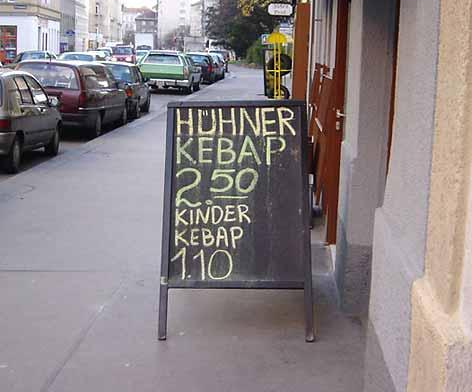
\includegraphics[scale=.55]{material/05Morph-Kebap}
\end{figure}

\end{frame}


%%%%%%%%%%%%%%%%%%%%%%%%%%%%%%%%%%
%%%%%%%%%%%%%%%%%%%%%%%%%%%%%%%%%%
\subsubsection{Rektionskomposita}
%\frame{
%\frametitle{~}
%	\tableofcontents[currentsection]
%}


%%%%%%%%%%%%%%%%%%%%%%%%%%%%%%%%%%
\begin{frame}
\frametitle{Rektionskomposita}

\begin{itemize}
	\item Wichtige \textbf{Untergruppe} der Determinativkomposita:
	
	\ea \label{ex:Bsp1} die Linguisten tagen – die Tagung der Linguisten – Linguistentagung
	\z
	
	\ea \label{ex:Bsp2} die Linguisten besteigen den Watzmann – die Besteigung des Watzmann – Watzmannbesteigung
	\z
		 
\end{itemize}


\end{frame}


%%%%%%%%%%%%%%%%%%%%%%%%%%%%%%%%%%
\begin{frame}
\frametitle{Rektionskomposita}

\begin{itemize}
	\item \textbf{deverbale} Nomina (durch Derivation)
	
	\begin{itemize}
		\item[]
		\item tagen \ras Tagung
		\item[]
		\item Verb bestimmt mit wie vielen und mit welchen Argumenten es im Satz erscheint (s. Rektion, Subkategorisierungsrahmen)
		
		\begin{itemize}
			\item[]
			\item Tagen in \ref{ex:Bsp1} + Subjekt
			\item[]
			\item besteigen in \ref{ex:Bsp2} + Subject + Objekt
			\item[]
			\item Beziehung zwischen Verb und seinen Argumenten auch innerhalb eines Kompositums
		\end{itemize}
	\end{itemize}
\end{itemize}


\end{frame}


%%%%%%%%%%%%%%%%%%%%%%%%%%%%%%%%%%
\begin{frame}
\frametitle{Rektionskomposita}

\begin{itemize}
	\item Rektionskompositum: \\
	die erste Konstituente in einem deverbalen Rektionskompositum realisiert ein Argument des der zweiten Konstituente zugrunde liegenden Verbs
	
	\begin{itemize}
		\item[]
		\item In \ref{ex:Bsp1}: \emph{Linguist(en)} \ras Subjekt von \emph{tagen}
		\item[]
		\item In \ref{ex:Bsp2}: Watzmann \ras Objekt von besteigen
	\end{itemize}
	
	\ea	 Auto$\cdot$fahrer (jemand fährt Auto), \\
		 Wetter$\cdot$beobachter (jemand beobachtet das Wetter), \\
		 Rotkehlchen$\cdot$gesang (das Rotkehlchen singt)
	\z
		 
\end{itemize}


\end{frame}


%%%%%%%%%%%%%%%%%%%%%%%%%%%%%%%%%%
\begin{frame}
\frametitle{Rektionskomposita}

\begin{itemize}
	\item Es gibt auch Rektionskomposita, in denen die zweite Konstituente ein nicht-deverbales Nomen oder ein Adjektiv ist, denn auch Nomina und Adjektive können Argumente nehmen:
	
	\ea Prüfungsangst (Angst vor der Prüfung), \\
		 Todessehnsucht (Sehnsucht nach dem Tod)
	\z
		 
	\ea staatstreu (dem Staat treu), \\
		 fälschungssicher (vor Fälschung sicher), \\
		 bleifrei (von Blei frei)
	\z
		 
\end{itemize}


\end{frame}


%%%%%%%%%%%%%%%%%%%%%%%%%%%%%%%%%%
\begin{frame}
\frametitle{Rektionskomposita}

\begin{itemize}
	\item \textbf{Rektionskompositum:} \\
	Kompositum, bei dem die \textbf{erste Konstituente ein Argument} (Subj., Akk.-Obj., Dat.-Obj., Gen.-Obj., Präp.-Obj., etc.) der zweiten Konstituente ist.
	\item[]
	\item Bei Nicht-Rektionskomposita besteht keine Argumentrelation.
	\item[]
	\item[] \textbf{ÜB.4}
	
\end{itemize}


\end{frame}


%%%%%%%%%%%%%%%%%%%%%%%%%%%%%%%%%%
%%%%%%%%%%%%%%%%%%%%%%%%%%%%%%%%%%
\subsubsection{Possessivkomposita}
%\frame{
%\frametitle{~}
%	\tableofcontents[currentsection]
%}


%%%%%%%%%%%%%%%%%%%%%%%%%%%%%%%%%%
\begin{frame}
\frametitle{Possessivkomposita}

\begin{itemize}
	\item Auch bei Possessivkomposita bestimmt die erste Konstituente die zweite näher.
	\item[]
	\item Das Kompositum bezieht sich aber auf \textbf{eine dritte Entität}, sie sind \textbf{exozentrisch}
	
	\ea \emph{Rot$\cdot$kehlchen} = Vogel, der ein rotes Kehlchen hat, nicht ein rotes Kehlchen ist
	\z
	
	\ea \emph{Rot$\cdot$käppchen} = Person, die eine rote Kappe hat (Märchenfigur), kein Käppchen
	\z
	
	\ea \emph{Lang$\cdot$finger} = Person, die lange Finger hat (= die stiehlt), kein Finger
	\z
	
\end{itemize}


\end{frame}


%%%%%%%%%%%%%%%%%%%%%%%%%%%%%%%%%%
%%%%%%%%%%%%%%%%%%%%%%%%%%%%%%%%%%
\subsubsection{Kopulativkomposita}
%\frame{
%\frametitle{~}
%	\tableofcontents[currentsection]
%}


%%%%%%%%%%%%%%%%%%%%%%%%%%%%%%%%%%
\begin{frame}
\frametitle{Kopulativkomposita}

\begin{itemize}
	\item Erste Konstituente \textbf{bestimmt} die zweite \textbf{nicht näher}
	\item[]
	\item Beide Konstituenten sind \textbf{gleichrangig}
	\item[]
	\item Auch aus mehr als zwei Konstituenten bestehend
	\item[]
	\item \textbf{Koordinierende} (= verknüpfende) Beziehung zwischen den Kompositionsgliedern
	\item[]
	\item Bedeutung des Kompositums ergibt sich \textbf{additiv}
	
	\eal 
	\ex süß$\cdot$sauer, nass$\cdot$kalt, rot$\cdot$grün, Fürst-Bischof
	\ex rot-rot-grün
	\zl
	
\end{itemize}


\end{frame}


%%%%%%%%%%%%%%%%%%%%%%%%%%%%%%%%%%
\begin{frame}
\frametitle{Kopulativkomposita}

\begin{itemize}
	\item Konstituenten in Kopulativkomposita \ras \textbf{gleiche Kategorie}
	\item[]
	\item Reihenfolge: prinzipiell frei, aber meistens \textbf{konventionalisiert}
	\item[]
	\item Anderes \textbf{Betonungsmuster} als Determinativkomposita
	
	\ea ein 'blau-'grünes 'Hemd - Kopulativ \\
		 ein 'blaugrünes 'Hemd - Determinativ
	\z
		 
	\item Während bei Determinativkomposita der Nichtkopf betont wird,\\
              werden bei Kopulativkomposita alle Konstituenten betont.
	\item[]
	\item[] \textbf{ÜB.5}
\end{itemize}


\end{frame}


%%%%%%%%%%%%%%%%%%%%%%%%%%%%%%%%%%
%%%%%%%%%%%%%%%%%%%%%%%%%%%%%%%%%%
\subsection{Wortstrukturregeln}
%\frame{
%\frametitle{~}
%	\tableofcontents[currentsection]
%}


%%%%%%%%%%%%%%%%%%%%%%%%%%%%%%%%%%
\begin{frame}
\frametitle{Wortstrukturregeln}

\begin{itemize}
	\item Unter Berücksichtigung der \textbf{Rechtsköpfigkeit} bei der Wortbildung gilt für Determinativ- und Possessivkomposita die folgende Wortbildungsregel:
	\item[]
	\item X \ras Y X
	\item[]
	\item wobei \gqq{X} und \gqq{Y} für \gqq{N}, \gqq{V}, \gqq{A} und \gqq{P} stehen, also:
	\item[]
	\item V \ras Y V'; N \ras Y N' usw.
	\item 	
	\item Für Kopulativkomposita gilt: alle Konstituenten sind von derselben Kategorie, also:
	\item[]
	\item N \ras N N 
\end{itemize}


\end{frame}


%%%%%%%%%%%%%%%%%%%%%%%%%%%%%%%%%%
\begin{frame}
\frametitle{Wortstrukturregeln}

\begin{itemize}
	\item Kopulativkomposita können mehr als zwei Glieder haben!
	\item Einige der Kompositionsregeln (aber nicht alle) sind \textbf{rekursiv}, d.h. sie können auf das Ergebnis einer Regelanwendung erneut angewendet werden, damit können im Prinzip unendlich lange Wörter gebildet werden:
	
	\begin{itemize}
		\item N+N-Komposita: (Struktur ist immer binär)
		\item[]
		\item Es gibt symmetrisch strukturierte (\textbf{beidseitigverzweigende}) Komposita \ref{ex:Bsp3}, \textbf{linksverzweigende} \ref{ex:Bsp4} und \textbf{rechtsverzweigende} \ref{ex:Bsp5}
		
		\ea \label{ex:Bsp3} ((Groß$\cdot$raum)$\cdot$(flug$\cdot$zeug))
		\z
		
		\ea \label{ex:Bsp4} (((Berb$\cdot$bau)$\cdot$(wissenschaft$\cdot$s)$\cdot$studium)
		\z
		
		\ea \label{ex:Bsp5} (Bezirk$\cdot$s$\cdot$(jahr$\cdot$es$\cdot$(haupt$\cdot$versammlung)))
		\z
		
	\end{itemize}
\end{itemize}


\end{frame}


%%%%%%%%%%%%%%%%%%%%%%%%%%%%%%%%%%
\begin{frame}
\frametitle{Wortstrukturregeln}

\begin{itemize}
	\item Komposita können auch strukturell ambig sein (\ref{ex:Bsp6} und \ref{ex:Bsp7})
	
	\ea\label{ex:Bsp6} ((Bund$\cdot$es$\cdot$straße$\cdot$n)$\cdot$bau) \vs \emph{(Bund$\cdot$es$\cdot$(straße$\cdot$n$\cdot$bau))}
	\z
	
	\ea \label{ex:Bsp7} ((Frau$\cdot$en$\cdot$film)$\cdot$fest) \vs (Frau$\cdot$en$\cdot$(film$\cdot$fest))
	\z
	
\end{itemize}


\begin{minipage}{.48\textwidth}

\begin{figure}
\centering
\scalebox{.7}{
\begin{forest}
sm edges,
	[N
		[N
			[N
				[Frau(en)]]
			[N
				[film]]]
		[N
			[fest]]]
\end{forest}}
\end{figure}

\end{minipage}\hfill%
\begin{minipage}{.48\textwidth}

\begin{figure}
\centering
\scalebox{.7}{
\begin{forest}
sm edges,
	[N
		[N
			[Frau(en)]]
		[N
			[N
				[film]]
			[N
				[fest]]]]
\end{forest}}
\end{figure}

\end{minipage}


\end{frame}


%%%%%%%%%%%%%%%%%%%%%%%%%%%%%%%%%%
\begin{frame}
\frametitle{Wortstrukturregeln}

\begin{itemize}
	\item Mit Verzweigungsrichtung (bei Determinativkomposita) \ras spezielle \textbf{Betonungsmuster}
	\item[]
	\item Bei \textbf{zweigliedrigen} Determinativkomposita wird generell der \textbf{Nichtkopf} betont.
	\item Bei \textbf{mehrgliedrigen} trägt meist der \textbf{Nichtkopf} der verzweigenden Konstituente den Hauptakzent
	\item Bei \textbf{symmetrisch} verzweigenden erhält die linke Konstituente den Hauptakzent:
	
	\ea (('Bundes$\cdot$es$\cdot$straße$\cdot$n)$\cdot$bau) \vs (Bund$\cdot$es$\cdot$('straße$\cdot$n$\cdot$bau))
	\z
	
	\ea '((Großraum)$\cdot$(flugzeug))
	\z
	
\end{itemize}


\end{frame}


%%%%%%%%%%%%%%%%%%%%%%%%%%%%%%%%%%%
%%%%%%%%%%%%%%%%%%%%%%%%%%%%%%%%%%%
%\section{X}
%%\frame{
%%\frametitle{~}
%%	\tableofcontents[currentsection]
%%}
%
%
%%%%%%%%%%%%%%%%%%%%%%%%%%%%%%%%%%%
%\begin{frame}
%\frametitle{Y}
%
%\begin{itemize}
%	\item 
%\end{itemize}
%
%
%\end{frame}


%%%%%%%%%%%%%%%%%%%%%%%%%%%%%%%%%%%
%%%%%%%%%%%%%%%%%%%%%%%%%%%%%%%%%%%
%\section{X}
%%\frame{
%%\frametitle{~}
%%	\tableofcontents[currentsection]
%%}
%
%
%%%%%%%%%%%%%%%%%%%%%%%%%%%%%%%%%%%
%\begin{frame}
%\frametitle{Y}
%
%\begin{itemize}
%	\item 
%\end{itemize}
%
%
%\end{frame}


%%%%%%%%%%%%%%%%%%%%%%%%%%%%%%%%%%%
%%%%%%%%%%%%%%%%%%%%%%%%%%%%%%%%%%%
%\section{X}
%%\frame{
%%\frametitle{~}
%%	\tableofcontents[currentsection]
%%}
%
%
%%%%%%%%%%%%%%%%%%%%%%%%%%%%%%%%%%%
%\begin{frame}
%\frametitle{Y}
%
%\begin{itemize}
%	\item 
%\end{itemize}
%
%
%\end{frame}


%%%%%%%%%%%%%%%%%%%%%%%%%%%%%%%%%%%
%%%%%%%%%%%%%%%%%%%%%%%%%%%%%%%%%%%
%\section{X}
%%\frame{
%%\frametitle{~}
%%	\tableofcontents[currentsection]
%%}
%
%
%%%%%%%%%%%%%%%%%%%%%%%%%%%%%%%%%%%
%\begin{frame}
%\frametitle{Y}
%
%\begin{itemize}
%	\item 
%\end{itemize}
%
%
%\end{frame}


%%%%%%%%%%%%%%%%%%%%%%%%%%%%%%%%%%%
%%%%%%%%%%%%%%%%%%%%%%%%%%%%%%%%%%%
%\section{X}
%%\frame{
%%\frametitle{~}
%%	\tableofcontents[currentsection]
%%}
%
%
%%%%%%%%%%%%%%%%%%%%%%%%%%%%%%%%%%%
%\begin{frame}
%\frametitle{Y}
%
%\begin{itemize}
%	\item 
%\end{itemize}
%
%
%\end{frame}


%%%%%%%%%%%%%%%%%%%%%%%%%%%%%%%%%%%
%%%%%%%%%%%%%%%%%%%%%%%%%%%%%%%%%%%
%\section{X}
%%\frame{
%%\frametitle{~}
%%	\tableofcontents[currentsection]
%%}
%
%
%%%%%%%%%%%%%%%%%%%%%%%%%%%%%%%%%%%
%\begin{frame}
%\frametitle{Y}
%
%\begin{itemize}
%	\item 
%\end{itemize}
%
%
%\end{frame}


%%%%%%%%%%%%%%%%%%%%%%%%%%%%%%%%%%%
%%%%%%%%%%%%%%%%%%%%%%%%%%%%%%%%%%%
%\section{X}
%%\frame{
%%\frametitle{~}
%%	\tableofcontents[currentsection]
%%}
%
%
%%%%%%%%%%%%%%%%%%%%%%%%%%%%%%%%%%%
%\begin{frame}
%\frametitle{Y}
%
%\begin{itemize}
%	\item 
%\end{itemize}
%
%
%\end{frame}


%%%%%%%%%%%%%%%%%%%%%%%%%%%%%%%%%%%
%%%%%%%%%%%%%%%%%%%%%%%%%%%%%%%%%%%
%\section{X}
%%\frame{
%%\frametitle{~}
%%	\tableofcontents[currentsection]
%%}
%
%
%%%%%%%%%%%%%%%%%%%%%%%%%%%%%%%%%%%
%\begin{frame}
%\frametitle{Y}
%
%\begin{itemize}
%	\item 
%\end{itemize}
%
%
%\end{frame}


%%%%%%%%%%%%%%%%%%%%%%%%%%%%%%%%%%%
%%%%%%%%%%%%%%%%%%%%%%%%%%%%%%%%%%%
%\section{X}
%%\frame{
%%\frametitle{~}
%%	\tableofcontents[currentsection]
%%}
%
%
%%%%%%%%%%%%%%%%%%%%%%%%%%%%%%%%%%%
%\begin{frame}
%\frametitle{Y}
%
%\begin{itemize}
%	\item 
%\end{itemize}
%
%
%\end{frame}


%%%%%%%%%%%%%%%%%%%%%%%%%%%%%%%%%%%
%%%%%%%%%%%%%%%%%%%%%%%%%%%%%%%%%%%
%\section{X}
%%\frame{
%%\frametitle{~}
%%	\tableofcontents[currentsection]
%%}
%
%
%%%%%%%%%%%%%%%%%%%%%%%%%%%%%%%%%%%
%\begin{frame}
%\frametitle{Y}
%
%\begin{itemize}
%	\item 
%\end{itemize}
%
%
%\end{frame}


%%%%%%%%%%%%%%%%%%%%%%%%%%%%%%%%%%%
%%%%%%%%%%%%%%%%%%%%%%%%%%%%%%%%%%%
%\section{X}
%%\frame{
%%\frametitle{~}
%%	\tableofcontents[currentsection]
%%}
%
%
%%%%%%%%%%%%%%%%%%%%%%%%%%%%%%%%%%%
%\begin{frame}
%\frametitle{Y}
%
%\begin{itemize}
%	\item 
%\end{itemize}
%
%
%\end{frame}


%%%%%%%%%%%%%%%%%%%%%%%%%%%%%%%%%%%
%%%%%%%%%%%%%%%%%%%%%%%%%%%%%%%%%%%
%\section{X}
%%\frame{
%%\frametitle{~}
%%	\tableofcontents[currentsection]
%%}
%
%
%%%%%%%%%%%%%%%%%%%%%%%%%%%%%%%%%%%
%\begin{frame}
%\frametitle{Y}
%
%\begin{itemize}
%	\item 
%\end{itemize}
%
%
%\end{frame}


%%%%%%%%%%%%%%%%%%%%%%%%%%%%%%%%%%%
%%%%%%%%%%%%%%%%%%%%%%%%%%%%%%%%%%%
%\section{X}
%%\frame{
%%\frametitle{~}
%%	\tableofcontents[currentsection]
%%}
%
%
%%%%%%%%%%%%%%%%%%%%%%%%%%%%%%%%%%%
%\begin{frame}
%\frametitle{Y}
%
%\begin{itemize}
%	\item 
%\end{itemize}
%
%
%\end{frame}


%%%%%%%%%%%%%%%%%%%%%%%%%%%%%%%%%%%
%%%%%%%%%%%%%%%%%%%%%%%%%%%%%%%%%%%
%\section{X}
%%\frame{
%%\frametitle{~}
%%	\tableofcontents[currentsection]
%%}
%
%
%%%%%%%%%%%%%%%%%%%%%%%%%%%%%%%%%%%
%\begin{frame}
%\frametitle{Y}
%
%\begin{itemize}
%	\item 
%\end{itemize}
%
%
%\end{frame}


%%%%%%%%%%%%%%%%%%%%%%%%%%%%%%%%%%%
%%%%%%%%%%%%%%%%%%%%%%%%%%%%%%%%%%%
%\section{X}
%%\frame{
%%\frametitle{~}
%%	\tableofcontents[currentsection]
%%}
%
%
%%%%%%%%%%%%%%%%%%%%%%%%%%%%%%%%%%%
%\begin{frame}
%\frametitle{Y}
%
%\begin{itemize}
%	\item 
%\end{itemize}
%
%
%\end{frame}


%%%%%%%%%%%%%%%%%%%%%%%%%%%%%%%%%%%
%%%%%%%%%%%%%%%%%%%%%%%%%%%%%%%%%%%
%\section{X}
%%\frame{
%%\frametitle{~}
%%	\tableofcontents[currentsection]
%%}
%
%
%%%%%%%%%%%%%%%%%%%%%%%%%%%%%%%%%%%
%\begin{frame}
%\frametitle{Y}
%
%\begin{itemize}
%	\item 
%\end{itemize}
%
%
%\end{frame}


%%%%%%%%%%%%%%%%%%%%%%%%%%%%%%%%%%%
%%%%%%%%%%%%%%%%%%%%%%%%%%%%%%%%%%%
%\section{X}
%%\frame{
%%\frametitle{~}
%%	\tableofcontents[currentsection]
%%}
%
%
%%%%%%%%%%%%%%%%%%%%%%%%%%%%%%%%%%%
%\begin{frame}
%\frametitle{Y}
%
%\begin{itemize}
%	\item 
%\end{itemize}
%
%
%\end{frame}


%%%%%%%%%%%%%%%%%%%%%%%%%%%%%%%%%%%
%%%%%%%%%%%%%%%%%%%%%%%%%%%%%%%%%%%
%\section{X}
%%\frame{
%%\frametitle{~}
%%	\tableofcontents[currentsection]
%%}
%
%
%%%%%%%%%%%%%%%%%%%%%%%%%%%%%%%%%%%
%\begin{frame}
%\frametitle{Y}
%
%\begin{itemize}
%	\item 
%\end{itemize}
%
%
%\end{frame}


%%%%%%%%%%%%%%%%%%%%%%%%%%%%%%%%%%%
%%%%%%%%%%%%%%%%%%%%%%%%%%%%%%%%%%%
%\section{X}
%%\frame{
%%\frametitle{~}
%%	\tableofcontents[currentsection]
%%}
%
%
%%%%%%%%%%%%%%%%%%%%%%%%%%%%%%%%%%%
%\begin{frame}
%\frametitle{Y}
%
%\begin{itemize}
%	\item 
%\end{itemize}
%
%
%\end{frame}


%%%%%%%%%%%%%%%%%%%%%%%%%%%%%%%%%%%
%%%%%%%%%%%%%%%%%%%%%%%%%%%%%%%%%%%
%\section{X}
%%\frame{
%%\frametitle{~}
%%	\tableofcontents[currentsection]
%%}
%
%
%%%%%%%%%%%%%%%%%%%%%%%%%%%%%%%%%%%
%\begin{frame}
%\frametitle{Y}
%
%\begin{itemize}
%	\item 
%\end{itemize}
%
%
%\end{frame}


%%%%%%%%%%%%%%%%%%%%%%%%%%%%%%%%%%%
%%%%%%%%%%%%%%%%%%%%%%%%%%%%%%%%%%%
%\section{X}
%%\frame{
%%\frametitle{~}
%%	\tableofcontents[currentsection]
%%}
%
%
%%%%%%%%%%%%%%%%%%%%%%%%%%%%%%%%%%%
%\begin{frame}
%\frametitle{Y}
%
%\begin{itemize}
%	\item 
%\end{itemize}
%
%
%\end{frame}


%%%%%%%%%%%%%%%%%%%%%%%%%%%%%%%%%%%
%%%%%%%%%%%%%%%%%%%%%%%%%%%%%%%%%%%
%\section{X}
%%\frame{
%%\frametitle{~}
%%	\tableofcontents[currentsection]
%%}
%
%
%%%%%%%%%%%%%%%%%%%%%%%%%%%%%%%%%%%
%\begin{frame}
%\frametitle{Y}
%
%\begin{itemize}
%	\item 
%\end{itemize}
%
%
%\end{frame}


%%%%%%%%%%%%%%%%%%%%%%%%%%%%%%%%%%%
%%%%%%%%%%%%%%%%%%%%%%%%%%%%%%%%%%%
%\section{X}
%%\frame{
%%\frametitle{~}
%%	\tableofcontents[currentsection]
%%}
%
%
%%%%%%%%%%%%%%%%%%%%%%%%%%%%%%%%%%%
%\begin{frame}
%\frametitle{Y}
%
%\begin{itemize}
%	\item 
%\end{itemize}
%
%
%\end{frame}


%%%%%%%%%%%%%%%%%%%%%%%%%%%%%%%%%%%
%%%%%%%%%%%%%%%%%%%%%%%%%%%%%%%%%%%
%\section{X}
%%\frame{
%%\frametitle{~}
%%	\tableofcontents[currentsection]
%%}
%
%
%%%%%%%%%%%%%%%%%%%%%%%%%%%%%%%%%%%
%\begin{frame}
%\frametitle{Y}
%
%\begin{itemize}
%	\item 
%\end{itemize}
%
%
%\end{frame}


%%%%%%%%%%%%%%%%%%%%%%%%%%%%%%%%%%%
%%%%%%%%%%%%%%%%%%%%%%%%%%%%%%%%%%%
%\section{X}
%%\frame{
%%\frametitle{~}
%%	\tableofcontents[currentsection]
%%}
%
%
%%%%%%%%%%%%%%%%%%%%%%%%%%%%%%%%%%%
%\begin{frame}
%\frametitle{Y}
%
%\begin{itemize}
%	\item 
%\end{itemize}
%
%
%\end{frame}


%%%%%%%%%%%%%%%%%%%%%%%%%%%%%%%%%%%
%%%%%%%%%%%%%%%%%%%%%%%%%%%%%%%%%%%
%\section{X}
%%\frame{
%%\frametitle{~}
%%	\tableofcontents[currentsection]
%%}
%
%
%%%%%%%%%%%%%%%%%%%%%%%%%%%%%%%%%%%
%\begin{frame}
%\frametitle{Y}
%
%\begin{itemize}
%	\item 
%\end{itemize}
%
%
%\end{frame}


%%%%%%%%%%%%%%%%%%%%%%%%%%%%%%%%%%%
%%%%%%%%%%%%%%%%%%%%%%%%%%%%%%%%%%%
%\section{X}
%%\frame{
%%\frametitle{~}
%%	\tableofcontents[currentsection]
%%}
%
%
%%%%%%%%%%%%%%%%%%%%%%%%%%%%%%%%%%%
%\begin{frame}
%\frametitle{Y}
%
%\begin{itemize}
%	\item 
%\end{itemize}
%
%
%\end{frame}


%%%%%%%%%%%%%%%%%%%%%%%%%%%%%%%%%%%
%%%%%%%%%%%%%%%%%%%%%%%%%%%%%%%%%%%
%\section{X}
%%\frame{
%%\frametitle{~}
%%	\tableofcontents[currentsection]
%%}
%
%
%%%%%%%%%%%%%%%%%%%%%%%%%%%%%%%%%%%
%\begin{frame}
%\frametitle{Y}
%
%\begin{itemize}
%	\item 
%\end{itemize}
%
%
%\end{frame}


%%%%%%%%%%%%%%%%%%%%%%%%%%%%%%%%%%%
%%%%%%%%%%%%%%%%%%%%%%%%%%%%%%%%%%%
%\section{X}
%%\frame{
%%\frametitle{~}
%%	\tableofcontents[currentsection]
%%}
%
%
%%%%%%%%%%%%%%%%%%%%%%%%%%%%%%%%%%%
%\begin{frame}
%\frametitle{Y}
%
%\begin{itemize}
%	\item 
%\end{itemize}
%
%
%\end{frame}


%%%%%%%%%%%%%%%%%%%%%%%%%%%%%%%%%%%
%%%%%%%%%%%%%%%%%%%%%%%%%%%%%%%%%%%
%\section{X}
%%\frame{
%%\frametitle{~}
%%	\tableofcontents[currentsection]
%%}
%
%
%%%%%%%%%%%%%%%%%%%%%%%%%%%%%%%%%%%
%\begin{frame}
%\frametitle{Y}
%
%\begin{itemize}
%	\item 
%\end{itemize}
%
%
%\end{frame}


%%%%%%%%%%%%%%%%%%%%%%%%%%%%%%%%%%%
%%%%%%%%%%%%%%%%%%%%%%%%%%%%%%%%%%%
%\section{X}
%%\frame{
%%\frametitle{~}
%%	\tableofcontents[currentsection]
%%}
%
%
%%%%%%%%%%%%%%%%%%%%%%%%%%%%%%%%%%%
%\begin{frame}
%\frametitle{Y}
%
%\begin{itemize}
%	\item 
%\end{itemize}
%
%
%\end{frame}


%%%%%%%%%%%%%%%%%%%%%%%%%%%%%%%%%%%
%%%%%%%%%%%%%%%%%%%%%%%%%%%%%%%%%%%
%\section{X}
%%\frame{
%%\frametitle{~}
%%	\tableofcontents[currentsection]
%%}
%
%
%%%%%%%%%%%%%%%%%%%%%%%%%%%%%%%%%%%
%\begin{frame}
%\frametitle{Y}
%
%\begin{itemize}
%	\item 
%\end{itemize}
%
%
%\end{frame}


%%%%%%%%%%%%%%%%%%%%%%%%%%%%%%%%%%%
%%%%%%%%%%%%%%%%%%%%%%%%%%%%%%%%%%%
%\section{X}
%%\frame{
%%\frametitle{~}
%%	\tableofcontents[currentsection]
%%}
%
%
%%%%%%%%%%%%%%%%%%%%%%%%%%%%%%%%%%%
%\begin{frame}
%\frametitle{Y}
%
%\begin{itemize}
%	\item 
%\end{itemize}
%
%
%\end{frame}


%%%%%%%%%%%%%%%%%%%%%%%%%%%%%%%%%%%
%%%%%%%%%%%%%%%%%%%%%%%%%%%%%%%%%%%
%\section{X}
%%\frame{
%%\frametitle{~}
%%	\tableofcontents[currentsection]
%%}
%
%
%%%%%%%%%%%%%%%%%%%%%%%%%%%%%%%%%%%
%\begin{frame}
%\frametitle{Y}
%
%\begin{itemize}
%	\item 
%\end{itemize}
%
%
%\end{frame}


%%%%%%%%%%%%%%%%%%%%%%%%%%%%%%%%%%%
%%%%%%%%%%%%%%%%%%%%%%%%%%%%%%%%%%%
%\section{X}
%%\frame{
%%\frametitle{~}
%%	\tableofcontents[currentsection]
%%}
%
%
%%%%%%%%%%%%%%%%%%%%%%%%%%%%%%%%%%%
%\begin{frame}
%\frametitle{Y}
%
%\begin{itemize}
%	\item 
%\end{itemize}
%
%
%\end{frame}


%%%%%%%%%%%%%%%%%%%%%%%%%%%%%%%%%%%
%%%%%%%%%%%%%%%%%%%%%%%%%%%%%%%%%%%
%\section{X}
%%\frame{
%%\frametitle{~}
%%	\tableofcontents[currentsection]
%%}
%
%
%%%%%%%%%%%%%%%%%%%%%%%%%%%%%%%%%%%
%\begin{frame}
%\frametitle{Y}
%
%\begin{itemize}
%	\item 
%\end{itemize}
%
%
%\end{frame}



%%%%%%%%%%%%%%%%%%%%%%%%%%%%%%%%%%%
%%%%%%%%%%%%%%%%%%%%%%%%%%%%%%%%%%%
%\section{X}
%%\frame{
%%\frametitle{~}
%%	\tableofcontents[currentsection]
%%}
%
%
%%%%%%%%%%%%%%%%%%%%%%%%%%%%%%%%%%%
%\begin{frame}
%\frametitle{Y}
%
%\begin{itemize}
%	\item 
%\end{itemize}
%
%
%\end{frame}


%%%%%%%%%%%%%%%%%%%%%%%%%%%%%%%%%%%
%%%%%%%%%%%%%%%%%%%%%%%%%%%%%%%%%%%
%\section{X}
%%\frame{
%%\frametitle{~}
%%	\tableofcontents[currentsection]
%%}
%
%
%%%%%%%%%%%%%%%%%%%%%%%%%%%%%%%%%%%
%\begin{frame}
%\frametitle{Y}
%
%\begin{itemize}
%	\item 
%\end{itemize}
%
%
%\end{frame}


%%%%%%%%%%%%%%%%%%%%%%%%%%%%%%%%%%%
%%%%%%%%%%%%%%%%%%%%%%%%%%%%%%%%%%%
%\section{X}
%%\frame{
%%\frametitle{~}
%%	\tableofcontents[currentsection]
%%}
%
%
%%%%%%%%%%%%%%%%%%%%%%%%%%%%%%%%%%%
%\begin{frame}
%\frametitle{Y}
%
%\begin{itemize}
%	\item 
%\end{itemize}
%
%
%\end{frame}


%%%%%%%%%%%%%%%%%%%%%%%%%%%%%%%%%%%
%%%%%%%%%%%%%%%%%%%%%%%%%%%%%%%%%%%
%\section{X}
%%\frame{
%%\frametitle{~}
%%	\tableofcontents[currentsection]
%%}
%
%
%%%%%%%%%%%%%%%%%%%%%%%%%%%%%%%%%%%
%\begin{frame}
%\frametitle{Y}
%
%\begin{itemize}
%	\item 
%\end{itemize}
%
%
%\end{frame}


%%%%%%%%%%%%%%%%%%%%%%%%%%%%%%%%%%%
%%%%%%%%%%%%%%%%%%%%%%%%%%%%%%%%%%%
%\section{X}
%%\frame{
%%\frametitle{~}
%%	\tableofcontents[currentsection]
%%}
%
%
%%%%%%%%%%%%%%%%%%%%%%%%%%%%%%%%%%%
%\begin{frame}
%\frametitle{Y}
%
%\begin{itemize}
%	\item 
%\end{itemize}
%
%
%\end{frame}


%%%%%%%%%%%%%%%%%%%%%%%%%%%%%%%%%%%
%%%%%%%%%%%%%%%%%%%%%%%%%%%%%%%%%%%
%\section{X}
%%\frame{
%%\frametitle{~}
%%	\tableofcontents[currentsection]
%%}
%
%
%%%%%%%%%%%%%%%%%%%%%%%%%%%%%%%%%%%
%\begin{frame}
%\frametitle{Y}
%
%\begin{itemize}
%	\item 
%\end{itemize}
%
%
%\end{frame}


%%%%%%%%%%%%%%%%%%%%%%%%%%%%%%%%%%%
%%%%%%%%%%%%%%%%%%%%%%%%%%%%%%%%%%%
%\section{X}
%%\frame{
%%\frametitle{~}
%%	\tableofcontents[currentsection]
%%}
%
%
%%%%%%%%%%%%%%%%%%%%%%%%%%%%%%%%%%%
%\begin{frame}
%\frametitle{Y}
%
%\begin{itemize}
%	\item 
%\end{itemize}
%
%
%\end{frame}


%%%%%%%%%%%%%%%%%%%%%%%%%%%%%%%%%%%
%%%%%%%%%%%%%%%%%%%%%%%%%%%%%%%%%%%
%\section{X}
%%\frame{
%%\frametitle{~}
%%	\tableofcontents[currentsection]
%%}
%
%
%%%%%%%%%%%%%%%%%%%%%%%%%%%%%%%%%%%
%\begin{frame}
%\frametitle{Y}
%
%\begin{itemize}
%	\item 
%\end{itemize}
%
%
%\end{frame}


%%%%%%%%%%%%%%%%%%%%%%%%%%%%%%%%%%%
%%%%%%%%%%%%%%%%%%%%%%%%%%%%%%%%%%%
%\section{X}
%%\frame{
%%\frametitle{~}
%%	\tableofcontents[currentsection]
%%}
%
%
%%%%%%%%%%%%%%%%%%%%%%%%%%%%%%%%%%%
%\begin{frame}
%\frametitle{Y}
%
%\begin{itemize}
%	\item 
%\end{itemize}
%
%
%\end{frame}


%%%%%%%%%%%%%%%%%%%%%%%%%%%%%%%%%%%
%%%%%%%%%%%%%%%%%%%%%%%%%%%%%%%%%%%
%\section{X}
%%\frame{
%%\frametitle{~}
%%	\tableofcontents[currentsection]
%%}
%
%
%%%%%%%%%%%%%%%%%%%%%%%%%%%%%%%%%%%
%\begin{frame}
%\frametitle{Y}
%
%\begin{itemize}
%	\item 
%\end{itemize}
%
%
%\end{frame}


%%%%%%%%%%%%%%%%%%%%%%%%%%%%%%%%%%%
%%%%%%%%%%%%%%%%%%%%%%%%%%%%%%%%%%%
%\section{X}
%%\frame{
%%\frametitle{~}
%%	\tableofcontents[currentsection]
%%}
%
%
%%%%%%%%%%%%%%%%%%%%%%%%%%%%%%%%%%%
%\begin{frame}
%\frametitle{Y}
%
%\begin{itemize}
%	\item 
%\end{itemize}
%
%
%\end{frame}


%%%%%%%%%%%%%%%%%%%%%%%%%%%%%%%%%%%
%%%%%%%%%%%%%%%%%%%%%%%%%%%%%%%%%%%
%\section{X}
%%\frame{
%%\frametitle{~}
%%	\tableofcontents[currentsection]
%%}
%
%
%%%%%%%%%%%%%%%%%%%%%%%%%%%%%%%%%%%
%\begin{frame}
%\frametitle{Y}
%
%\begin{itemize}
%	\item 
%\end{itemize}
%
%
%\end{frame}


%%%%%%%%%%%%%%%%%%%%%%%%%%%%%%%%%%%
%%%%%%%%%%%%%%%%%%%%%%%%%%%%%%%%%%%
%\section{X}
%%\frame{
%%\frametitle{~}
%%	\tableofcontents[currentsection]
%%}
%
%
%%%%%%%%%%%%%%%%%%%%%%%%%%%%%%%%%%%
%\begin{frame}
%\frametitle{Y}
%
%\begin{itemize}
%	\item 
%\end{itemize}
%
%
%\end{frame}


%%%%%%%%%%%%%%%%%%%%%%%%%%%%%%%%%%%
%%%%%%%%%%%%%%%%%%%%%%%%%%%%%%%%%%%
%\section{X}
%%\frame{
%%\frametitle{~}
%%	\tableofcontents[currentsection]
%%}
%
%
%%%%%%%%%%%%%%%%%%%%%%%%%%%%%%%%%%%
%\begin{frame}
%\frametitle{Y}
%
%\begin{itemize}
%	\item 
%\end{itemize}
%
%
%\end{frame}


%%%%%%%%%%%%%%%%%%%%%%%%%%%%%%%%%%%
%%%%%%%%%%%%%%%%%%%%%%%%%%%%%%%%%%%
%\section{X}
%%\frame{
%%\frametitle{~}
%%	\tableofcontents[currentsection]
%%}
%
%
%%%%%%%%%%%%%%%%%%%%%%%%%%%%%%%%%%%
%\begin{frame}
%\frametitle{Y}
%
%\begin{itemize}
%	\item 
%\end{itemize}
%
%
%\end{frame}


%%%%%%%%%%%%%%%%%%%%%%%%%%%%%%%%%%%
%%%%%%%%%%%%%%%%%%%%%%%%%%%%%%%%%%%
%\section{X}
%%\frame{
%%\frametitle{~}
%%	\tableofcontents[currentsection]
%%}
%
%
%%%%%%%%%%%%%%%%%%%%%%%%%%%%%%%%%%%
%\begin{frame}
%\frametitle{Y}
%
%\begin{itemize}
%	\item 
%\end{itemize}
%
%
%\end{frame}


%%%%%%%%%%%%%%%%%%%%%%%%%%%%%%%%%%%
%%%%%%%%%%%%%%%%%%%%%%%%%%%%%%%%%%%
%\section{X}
%%\frame{
%%\frametitle{~}
%%	\tableofcontents[currentsection]
%%}
%
%
%%%%%%%%%%%%%%%%%%%%%%%%%%%%%%%%%%%
%\begin{frame}
%\frametitle{Y}
%
%\begin{itemize}
%	\item 
%\end{itemize}
%
%
%\end{frame}


%%%%%%%%%%%%%%%%%%%%%%%%%%%%%%%%%%%
%%%%%%%%%%%%%%%%%%%%%%%%%%%%%%%%%%%
%\section{X}
%%\frame{
%%\frametitle{~}
%%	\tableofcontents[currentsection]
%%}
%
%
%%%%%%%%%%%%%%%%%%%%%%%%%%%%%%%%%%%
%\begin{frame}
%\frametitle{Y}
%
%\begin{itemize}
%	\item 
%\end{itemize}
%
%
%\end{frame}


%%%%%%%%%%%%%%%%%%%%%%%%%%%%%%%%%%%
%%%%%%%%%%%%%%%%%%%%%%%%%%%%%%%%%%%
%\section{X}
%%\frame{
%%\frametitle{~}
%%	\tableofcontents[currentsection]
%%}
%
%
%%%%%%%%%%%%%%%%%%%%%%%%%%%%%%%%%%%
%\begin{frame}
%\frametitle{Y}
%
%\begin{itemize}
%	\item 
%\end{itemize}
%
%
%\end{frame}


%%%%%%%%%%%%%%%%%%%%%%%%%%%%%%%%%%%
%%%%%%%%%%%%%%%%%%%%%%%%%%%%%%%%%%%
%\section{X}
%%\frame{
%%\frametitle{~}
%%	\tableofcontents[currentsection]
%%}
%
%
%%%%%%%%%%%%%%%%%%%%%%%%%%%%%%%%%%%
%\begin{frame}
%\frametitle{Y}
%
%\begin{itemize}
%	\item 
%\end{itemize}
%
%
%\end{frame}


%%%%%%%%%%%%%%%%%%%%%%%%%%%%%%%%%%%
%%%%%%%%%%%%%%%%%%%%%%%%%%%%%%%%%%%
%\section{X}
%%\frame{
%%\frametitle{~}
%%	\tableofcontents[currentsection]
%%}
%
%
%%%%%%%%%%%%%%%%%%%%%%%%%%%%%%%%%%%
%\begin{frame}
%\frametitle{Y}
%
%\begin{itemize}
%	\item 
%\end{itemize}
%
%
%\end{frame}


%%%%%%%%%%%%%%%%%%%%%%%%%%%%%%%%%%%
%%%%%%%%%%%%%%%%%%%%%%%%%%%%%%%%%%%
%\section{X}
%%\frame{
%%\frametitle{~}
%%	\tableofcontents[currentsection]
%%}
%
%
%%%%%%%%%%%%%%%%%%%%%%%%%%%%%%%%%%%
%\begin{frame}
%\frametitle{Y}
%
%\begin{itemize}
%	\item 
%\end{itemize}
%
%
%\end{frame}


%%%%%%%%%%%%%%%%%%%%%%%%%%%%%%%%%%%
%%%%%%%%%%%%%%%%%%%%%%%%%%%%%%%%%%%
%\section{X}
%%\frame{
%%\frametitle{~}
%%	\tableofcontents[currentsection]
%%}
%
%
%%%%%%%%%%%%%%%%%%%%%%%%%%%%%%%%%%%
%\begin{frame}
%\frametitle{Y}
%
%\begin{itemize}
%	\item 
%\end{itemize}
%
%
%\end{frame}


%%%%%%%%%%%%%%%%%%%%%%%%%%%%%%%%%%%
%%%%%%%%%%%%%%%%%%%%%%%%%%%%%%%%%%%
%\section{X}
%%\frame{
%%\frametitle{~}
%%	\tableofcontents[currentsection]
%%}
%
%
%%%%%%%%%%%%%%%%%%%%%%%%%%%%%%%%%%%
%\begin{frame}
%\frametitle{Y}
%
%\begin{itemize}
%	\item 
%\end{itemize}
%
%
%\end{frame}




